%%%%%%%%%%%%%%%%%%%%%%%%%%%%%%%%%%%%%%%%%%%%%%%%%%%%%%%%%%%%%%%%%%%%%%%%%%%%%%
% Jan Kalina <xkalin03@stud.fit.vutbr.cz> 2013
%%%%%%%%%%%%%%%%%%%%%%%%%%%%%%%%%%%%%%%%%%%%%%%%%%%%%%%%%%%%%%%%%%%%%%%%%%%%%%

%%%%%%%%%%%%%%%%%%%%%%%%%%%%%%%%%%%%%%%%%%%%%%%%%%%%%%%%%%%%%%%%%%%%%%%%%%%%%%
\chapter{Bezpečnost v Javě} \label{teoretickyUvod}
%%%%%%%%%%%%%%%%%%%%%%%%%%%%%%%%%%%%%%%%%%%%%%%%%%%%%%%%%%%%%%%%%%%%%%%%%%%%%%

%=============================================================================
\section{Bezpečnost}
%=============================================================================

Protože se tato práce zabývá bezpečností, což je pojem, který lze v různých souvislostech chápat zcela odlišně, je nanejvýš vhodné nejprve specifikovat co termínem bezpečnosti míníme a z kterého pohledu se jí budeme zabývat.

Scott Oaks definuje ve své knize Java Security bezpečnost jako souhrn následujících kritérií: \cite[1.1]{oaks}

\begin{itemize}
  \item {\bf Bezpečí vůči zákeřnému software} -- programy by neměly být schopny poškodit prostředí hostitelského počítače.
  \item {\bf Bezpečí vůči Velkému bratru} -- programům by mělo být bráněno ve sledování uživatele -- programy by neměly být schopny svévolně číst soukromé informace na počítači na kterém běží, ani na síti ke které je tento počítač připojen.
  \item {\bf Autentizace} -- identita autorů programu by měla být ověřována (typicky pomocí digitálního podpisu).
  \item Šifrování -- data odesílaná a přijímaná programem by měla být šifrována.
  \item Auditovatelnost -- potenciálně škodlivé operace by měly být vždy zaznamenávány.
  \item Specifikovanost -- program by měla doprovázet specifikace bezpečnostních pravidel, které program dodržuje.
  \item Verifikovanost -- pro prováděné operace by měla být stanovena pravidla, proti kterým by měly být verifikovány.
  \item Dbaní na dobré vychování -- programům by mělo být bráněno v užívání příliš mnoha systémových prostředků.
\end{itemize}

V souvislosti s víceuživatelskými prostředími se pak pojem bezpečnosti vyskytuje ještě v další rovině, kdy nejde o bezpečí systému před běžící aplikací, ale o způsob jakým může naopak program ověřit, kdo je jeho uživatelem a zdali má právo po něm žádat vykonání operace, o jejíž vykonání žádá.

Tato práce se zabývá bezpečností ve smyslu prvních tří bodů uvedeného výčtu (uvedeny tučně). Bude se tedy zabývat způsobem ochrany prostředí hostitelského počítače před jeho poškozením nebo neoprávněným sledováním ze strany běžících programů. Právě oprávnění programu pak souvisí s autentizací. Autentizací se myslí ověřování autorství programu. Právě od toho, kdo je autorem programu, se totiž mohou oprávnění programu odvozovat.

%=============================================================================
\section{Java}
%=============================================================================

Programy v jazyce Java bývají překládány do platformě nezávislého a efektivněji než kód v jazyce Java interpretovatelného mezikódu, takzvaného bajtkódu.
Bajtkód ({\it Bytecode}) bývá zpravidla interpretován virtuálním strojem Javy (JVM - Java Virtual Machine).
JVM je abstraktní výpočetní stroj. Podobně jako reálné výpočetní stroje má svoji instrukční sadu a paměť se kterou může manipulovat, ale na rozdíl od nich pro něj neexistuje jeho fyzická implementace, pouze emulovaná implementace softwarová.
To znamená že její kód není prováděn nativně hardwarem, ale je interpretován speciálním programem, interpretem, který je sám zkompilován do nativního kódu dané platformy.
To mimo nezávislosti na platformě přináší také vyšší stupeň abstrakce.

Díky tomu, že programy nepřistupují ani nemohou přistupovat ke zdrojům fyzického stroje přímo, ale pouze zprostředkovaně skrze zdroje virtuální stroje Javy, si není těžké představit, že by použití takovéhoto virtuálního stroje mohlo mít i významný bezpečnostní efekt.
Protože programy v JVM mohou k fyzickým zdrojům počítače (např. k souborům nebo k síti) přistupovat jen skrze JVM, zablokování takového přístupu ze strany JVM není nikterak složité - JVM stačí odmítnout takový požadavek a interpretovaný program nemá možnost JVM obejít.

%=============================================================================
\section{Java security manager} \label{securityManager}
%=============================================================================

Pro maximální nastavitelnost omezení kladených na programy běžících na virtuálních strojích Javy nerozhoduje o povolení nebo zablokování operace nad zdrojem JVM samotná JVM, ale dotazuje se speciálního objektu třídy {\it java.lang.SecurityManager}, nebo jeho podtřídy.

Podtřída je třída dědící atributy a metody (operace, přijímané zprávy) své nadtřídy a reference na její instanci může být vložena do proměnné určené pro referenci na její nadtřídu. Jakákoli podtřída třídy {\it SecurityManager} tedy bude vždy přijímat všechny zprávy, které přijímá třída {\it SecurityManager}, přičemž ty, které nebude sama implementovat, budou přejaty z její nadtřídy {\it SecurityManager}.

Security manager, který JVM použije při svém startu lze ovlivnit skrze konfigurační proměnnou JVM -- {\it java.security.manager}. Za běhu je možné aktuálně používaný security manager zjistit voláním {\it System.getSecurityManager() } a vypnout nebo vyměnit voláním {\it System.setSecurityManager()}. Volání těchto metod je samo chráněno security managerem, takže nehrozí, že by se program neoprávněně zbavil omezení, které na něj uvalil security manager jeho vypnutím nebo výměnou.

Hodnotu konfigurační proměnné {\it java.security.manager} po startu JVM je možné nastavit za pomoci k tomu určeného parametru {\tt -D}. Pro spuštění programu s výchozím security managerem můžeme tedy použít příkaz:

\begin{verbatim}
java -Djava.security.manager=default ProgramABC
\end{verbatim}

Základní možné hodnoty proměnné {\it java.security.manager} a jim odpovídající třídy objektů security manageru popisuje následující tabulka.

\begin{table}[tb]
\label{parametryJavy}
\caption{popis tabulky}
\begin{center}
    \begin{tabular}{| l | l |}
    \hline
    Parametr příkazu java & Použitý JSM \\ \hline
    (parametr nepoužit)                                      & {\tt null                      } \\
    {\tt -Djava.security.manager                           } & {\tt java.lang.SecurityManager } \\
    {\tt -Djava.security.manager=default                   } & {\tt java.lang.SecurityManager } \\
    {\tt -Djava.security.manager=java.lang.SecurityManager } & {\tt java.lang.SecurityManager } \\
    {\tt -Djava.security.manager=TestovaciSM               } & {\tt TestovaciSM               } \\
    \hline
    \end{tabular}
\end{center}
\end{table}

TODO: Ostatní řádky?

Poslední řádek demonstruje použití vlastní třídy objektu security manageru. Způsob vytvoření vlastní třídy security manageru bude podrobněji rozebrán v další kapitole. Jestliže je zde uvedena neexistující třída, skončí inicializace JVM výjimkou a vykonávání programu nebude vůbec zahájeno:

\begin{lstlisting}[caption=Vyjímka při spuštění JVM s neexistujícím správcem bezpečnosti, label=smEx]
Error occurred during initialization of VM
java.lang.InternalError: Could not create SecurityManager: neexistujici.SM
    at sun.misc.Launcher.<init>(Launcher.java:106)
    at sun.misc.Launcher.<clinit>(Launcher.java:57)
    at java.lang.ClassLoader.initSystemClassLoader(ClassLoader.java:1486)
    at java.lang.ClassLoader.getSystemClassLoader(ClassLoader.java:1468)
\end{lstlisting}

Tím, že je zabráněno startu JVM v případě chybné konfigurace security manageru, je tedy uplatněn bezpečnostní princip, kdy systém zůstane bezpečný i v případě poruchového stavu.

%=============================================================================
\section{Implementace vlastního Security manageru}
%=============================================================================

V této podkapitole bude vysvětlen způsob stanovení bezpečnostní politiky vytvořením vlastního security manageru.
Security manager je objekt, na který JVM při požadavku na Java API deleguje rozhodnutí o povolení nebo nepovolení operace nad zdrojem.
Tento objekt musí být instancí třídy {\it java.lang.SecurityManager} nebo její podtřídy. \cite{tutorialsTSM}

Algoritmus používaný Java API pro rozhodnutí o vykonání nebo nevykonání potenciálně nebezpečné operace je následující: \cite[4.1.1]{oaks}

\begin{enumerate}
  \item Uživatelská aplikace žádá prostřednictvím Java API o provedení dané operace
  \item Java API se dotáže security manageru zda operaci povolit zavoláním patřičné metody security manageru.
  \item Nemá-li být operace povolena, vrátí Security manager výjimku {\it SecurityException}, která je předána uživatelské aplikaci, čímž je vykonání operace zabráněno.
  \item Není-li vyhozena žádná výjimka, operace se považuje za povolenou a je provedena.
\end{enumerate}

Vlastní Security manager tedy vytvoříme rozšířením třídy {\it SecurityManager}, přičemž přepíšeme metody rozhodující o povolení akce, kterou chceme povolit, nebo pro kterou chceme stanovit vlastní algoritmus rozhodující zda akci povolit nebo ne.
Protože standardní security manager implicitně všechny operace zakazuje, stačí nám implementovat metody autorizující provedení operací, které chceme povolit a operacemi které nikdy povolit chtít nebudeme se nebudeme muset zabývat.

Příklad níže ukazuje jednoduchý security manager, který o povolení každé akce rozhodne na základě interakce s uživatelem. Při pokusu programu o provedení potenciálně nebezpečné operace je uživateli zobrazen dotaz, zda chce tuto operaci povolit nebo ne. V případě negativní odpovědi je jejímu provedení vrácením výjimky {\it SecurityException} zabráněno.

\begin{lstlisting}[caption=Jednoduchý testovací správce bezpečnosti, label=TestovaciSM]
public class TestovaciSM extends SecurityManager {
	@Override
	public void checkPermission(Permission permission) {
		
		System.out.println("Povolit " + permission.toString() + " ?");
		if(!askUser()){ // jestlize uzivatel nezvoli "povolit"
			throw new SecurityException("Operace byla zakazana uzivatelem");
		}
		
	}
}
\end{lstlisting}

Takto vytvořený security manager pak můžeme na vlastní program nechat použít za pomoci dříve zmíněného příkazu:

\begin{verbatim}
System.setSecurityManager(new TestovaciSM());
\end{verbatim}

Jinak (pro libovolný program) můžeme použití tohoto security manageru nastavit při startu JVM:

\begin{verbatim}
java -Djava.security.manager=TestovaciSM HelloWorld
\end{verbatim}

Nutno dodat že tato konfigurační proměnná je uplatněna při startu JVM, její změnou za běhu JVM nebude použití security manageru ovlivněno.

Zde uvedený security manager je opravdu pouze demonstrativní, v čemž se můžeme utvrdit, spustíme-li jej nad jednoduchou aplikací Hello world. Na správce bezpečnosti bude i v tomto jednoduchém případě kladeno celkem 29 dotazů.

Jelikož samotný výpis textu na standardní výstup není operací kontrolovanou správcem bezpečnosti, je příčinou všech dotazů na správce bezpečnosti inicializace samotného virtuálního stroje Javy.

V 18 případech je příčinou dotazu čtení obsahu konfiguračních proměnných (Property), v 8 případech jde o manipulaci s vlákny (Thread) a ve zbývajících 3 případech jde o čtení samotného souboru spouštěné třídy ({\tt Program.class})

Množství dotazů kladených na správce bezpečnosti je tedy i u takto primitivní aplikace příliš velký, než aby bylo možné nechat je zodpovídat uživatelem a vytvořit tak správce bezpečnosti pracujícího na principu interaktivní protipožární přepážky (firewall).

Stanovení bezpečnostní politiky vytvořením security manageru ale nepochybně možné je. Vyžaduje ale znalosti programování v Javě od správce počítače na němž JVM běží a od Javy verze 2 se již pro stanovení bezpečnostní politiky nepoužívá.

%=============================================================================
\section{Zavaděče tříd}
%=============================================================================

Než se dostaneme k v současnosti využívanému způsobu stanovování bezpečnostní politiky, pozastavíme se nad tématem zavádění tříd.
Ačkoli se na první pohled může zdát, že toto téma s bezpečností příliš nesouvisí, opak je pravdou.
Jen a pouze zavaděč tříd (classloader), který třídu do paměti zavádí totiž může určit původ třídy, od kterého se oprávnění kódu této třídy odvozuje.

Zavaděč je objekt odpovědný za načítání tříd a rozhraní v Javě. Na základně binárního názvu třídy (tedy názvu používaného v bytekódu, např. {\it java.lang.String} nebo {\it java.security.KeyStore\$Builder\$FileBuilder\$1}) se pokusí vyhledat a načíst třídu daného názvu. \cite{refClassLoader}

Třída každého zavaděče musí být podtřídou třídy {\it java.lang.ClassLoader} a musí implementovat metodu {\it findClass()}, která provádí právě samotné vyhledání třídy podle názvu. Jejím výstupem je objekt třídy {\it Class} představující samotnou třídu. Při programování běžných aplikací můžeme na objekty této třídy narazit například při snaze získat název třídy neznámého objektu jako řetězec za běhu aplikace: \cite{refClassLoader}

\begin{verbatim}
Class tridaObjektuX = x.getClass();
String nazevTridyObjektuX = c.getName();
\end{verbatim}

Každý objekt v Javě si totiž uchovává referenci na svoji třídu, již zmíněný objekt třídy {\it Class}, obsahující mimo jiného také právě název třídy ve formě textového řetězce.

Jako původ třídy ({\it CodeSource}) souhrnně označujeme URL adresu, ze které byla třída získána, a elektronické podpisy, kterými přitom byl její JAR archiv opatřen.
Na základě původu je třída zařazena do ochranné domény. Mají-li dvě třídy stejný původ, je jim přiřazena stejná ochranná doména. \cite[5.1]{oaks}\cite{sourceSecureClassLoader}

Ochranná doména ({\it ProtectionDomain}) je uskupení zdrojových kódů a oprávnění, které jsou tomuto kódu udělena.
Speciálním případem je tzv. systémová ochranná doména, do které spadají třídy zavedení interním zavaděčem tříd (viz. \ref{interniZavadec}), jejíž reference na ochrannou doménu je nastavena na {\it null} a jejich oprávnění nejsou omezené. \cite[5.4]{oaks}

%-----------------------------------------------------------------------------
\subsection{Interní zavaděč tříd} \label{interniZavadec}
%-----------------------------------------------------------------------------

Interní zavaděč tříd je zavaděč používaný pro načítání tříd samotného Java API a zavaděčů uživatelských tříd.
Interní zavaděč je součástí JVM. Je napsán převážně v nativním kódu a k načítání tříd využívá nativní metody pro přístup k souborovému systému operačního systému.
Interní zavaděč načítá třídy ze souborů, jejíž adresu odvozuje z názvu třídy, balíčku a proměnné prostředí CLASSPATH. \cite[3.2.1]{oaks}

Je-li tedy JVM spuštěna následujícím příkazem:

\begin{verbatim}
java -classpath /srv/classes muj.program.Test
\end{verbatim}

Bude spuštěna třídní metoda {\it main()} třídy {\it Test}, jež bude hledána v souboru:

\begin{verbatim}
/srv/classes/muj/program/Test.class
\end{verbatim}

O třídách načtených interním zavaděčem se často mluví jako o třídách bez zavaděče, protože jejich objekt {\it Class} má referenci na zavaděč nastavenu na {\it null}. \cite[3.2.1]{oaks} Zároveň je {\it null}ová také ochranná doména takto načtených tříd. Třídy načtené interním zavaděčem tak nemají svá oprávnění omezena.

Interní zavaděč je v současnosti používán k načítání jen nejzákladnějších tříd, zejména tříd Java API, tedy tříd používajících součásti napsané v nativním kódu. Ostatní třídy z {\it CLASSPATH} jsou obvykle načítány Zavaděčem tříd z URL.

%-----------------------------------------------------------------------------
\subsection{Zavaděč tříd z URL}
%-----------------------------------------------------------------------------

Zavaděč tříd z URL ({\it URLClassLoader}) hledá třídy také na URL adresách určených polem objektů {\it URL}, předaných jeho konstruktoru. Je jedním z nejpoužívanějších zavaděčů tříd v Javě -- používá se i k vyhledávání méně základních tříd z {\it CLASSPATH} a dokáže třídy načítat nejen z adresářů, ale i z JAR archivů, je-li jako adresa uvedena adresa JAR archivu. \cite[3.2.5]{oaks}

\begin{verbatim}
URLClassLoader urlClassLoader = new URLClassLoader(new URL[]{
    new URL("http://server/directory/"),
    new URL("file:/srv/classes/")
}, parentClassloader);
\end{verbatim}

Zavaděč tříd z URL je jedním z bezpečných zavaděčů ({\it SecureClassLoader}). To znamená že automaticky nastavuje ochranou doménu třídám, které načítá.
Ochranná doména která bude zvolena závisí na následujících parametrech: \cite{refPolicyFiles}

\begin{itemize}
  \item {\tt codeBase}: URL adresa ze které byla třída načtena.
  \item {\tt signedBy}: Alias podpisu, kterým byl JAR archiv z něhož byla třída načtena podepsán.
  \item {\tt principal}: Operaci žádá kód spuštěný uživatelem s oprávněním uvedeným v pravidlu bezpečnostní politiky.
\end{itemize}

Třídy, které mají všechny tyto parametry společné, patří do stejné ochranné domény a mají tak stejná oprávnění.

%=============================================================================
\section{Access Controller a soubory bezpečnostní politiky}
%=============================================================================

Access controller je mechanismus využívající ochranné domény tříd, který standardní security manager (od Javy verze 2) využívá pro rozhodnutí, zda operaci požadovanou uživatelským programem povolit či nikoliv. Aby tedy byla aplikována omezení stanovená {\tt Access controller}em, musí být JVM spuštěna se standardním security managerem. \cite[5]{oaks}

Access controller, stejně jako security manager, umožňuje omezit, zdali může být operace nad zdrojem provedena nebo ne. Zdroji zda však již nejsou jen zdroje samotné JVM. Access controller mohou využívat i uživatelské procesy pro omezení přístupu ke zdrojům, které poskytují. \cite[5]{oaks}

Máme-li tedy knihovní třídu zprostředkovávající přístup k databázi v souboru po záznamech, při použití oprávnění jen na úrovni Java API by bylo možné programu přidělovat oprávnění jen k celému souboru. Access controller ale umožňuje považovat jednotlivé záznamy databáze v souboru za samostatné zdroje, čímž umožňuje různým programům přidělit oprávnění jen k vybraným záznamům v databázovém souboru.

Access controller je schopný pravidla bezpečnostní politiky načítat z textového konfiguračního souboru -- tzv. souboru bezpečnostní politiky. Vzniká tak mnohem snazší způsob stanovení bezpečnostní politiky, kterou budou programy v JVM omezeny -- namísto tvorby vlastní třídy security manageru bude pro stanovení bezpečnostní politiky stačit upravovat obsah souboru bezpečnostní politiky. \cite[5]{oaks}

Ochranná doména (Protection Domain) je uskupení zdrojových kódů a oprávnění, které jsou tomuto kódu udělena. Každá třída spadá vždy do jedné ochranné domény, která jí je přidělena zavaděčem při jejím načítání. Jen zavaděč totiž zná původ třídy, na základě kterého jsou třídy ochranným doménám přidělovány. Speciálním případem jsou třídy zavedené interním zavaděčem (viz. \ref{interniZavadec}), které spadají do systémové ochranné domény a mají tak vždy povoleno vše. \cite[5.4]{oaks}

Access controller rozhoduje o povolení nebo nepovolení operace na základně průniku oprávnění ochranných domén tříd metod, jež vedly k zavolání metody provádějící citlivou operaci. Na legálnost operace se access controlleru může dotazovat samotná volaná metoda (voláním metody {\it checkPermission()}), nebo security manager na základě dotazu na legálnost aplikace od Java API.

\begin{figure}[ht]
  \centering
  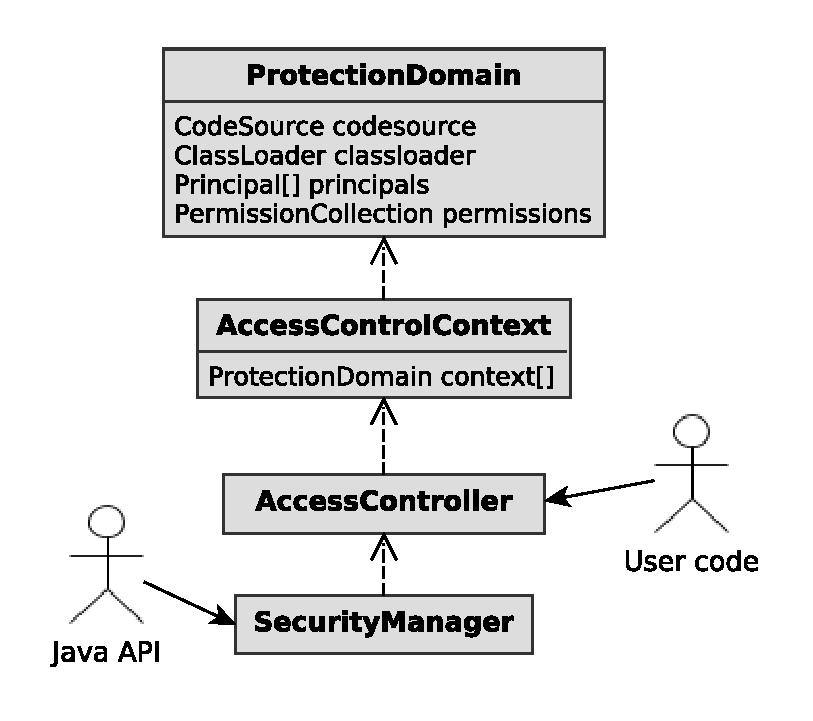
\includegraphics[width=10cm]{fig/security-schema}
  \caption{Schéma vzájemných souvislostí tříd zajišťujících bezpečnost v Javě}
\end{figure}

%-----------------------------------------------------------------------------
\subsection{Implementace Access Controlleru}\label{implementaceAC}
%-----------------------------------------------------------------------------

Access controller je implementován třídou {\it AccessController} a voláním jeho statických metod na něj standardní security manager deleguje rozhodnutí o legálnosti provedení potenciálně nežádoucí operace uživatelského programu. Konkrétně kontrolu obstarává metoda {\it checkPermission(Permission)}, která v případě neoprávněnosti požadavku na provedení operace způsobí vyhození výjimky {\it AccessControlException}. Jejím vstupem je objekt třídy {\it Permission}, která reprezentuje oprávnění, jehož vlastnictví je testováno. \cite[5.5]{oaks}\cite[6]{oaks}

Následující příklad ukazuje způsob, jakým se může kód dotázat Access controlleru, zdali má zadané oprávnění: \cite[5.5]{oaks}

\begin{verbatim}
try {
    // má tento program oprávnění připojit se na lokální port 80?
    AccessController.checkPermission(
        new SocketPermission("localhost:80", "connect")
    );
    System.out.println("Program má oprávnění připojit se na port");
} catch (AccessControlException ace) {
    System.out.println("Program nemá oprávnění připojit se na port");
}
\end{verbatim}

Access controller rozhoduje o povolení nebo nepovolení operace na základně průniku oprávnění ochranných domén tříd metod, jež vedly k zavolání metody {\it checkPermission()}. Konkrétně jde o metody nacházející se během volání {\it checkPermission()} na zásobníku volání (Stack trace). Volala-li tedy metoda {\it main} třídy {\it Main} metodu {\it secured} třídy {\it Secured}, která následně zavolala metodu {\it checkPermission()}, musí mít požadované oprávnění přiděleny ochranné domény tříd {\it Main} i {\it Secured}, aby toto volání neskončilo výjimkou vyjadřující zamítnutí provedení operace ze strany Access controlleru. \cite[5.5]{oaks}\cite[6.1]{oaks}


%Access controller je založen na čtyř konceptech: \cite[5]{oaks}
%
%\begin{itemize}
%  \item Zdroje kódu (CodeSource): Objekt představující původ třídy -- adresu URL z které byla získána a certifikáty (elektronické podpisy), kterými byla opatřena %\cite[5.1]{oaks}
%  \item Oprávnění (Permission): Objekt představující operaci o jejíž povolení se rozhoduje, konkrétně se skládá z trojice: typ oprávnění, název zdroje, povolené akce \cite[5.2]{oaks}
%  \item Politiky (Policy): Objekt představující souhrn oprávnění udělených danému zdrojovému kódu \cite[5.3]{oaks}
%  \item Ochranná doména (ProtectionDomain): Objekt představující zdrojové kódy a jejich oprávnění \cite[5.4]{oaks}
%\end{itemize}

%-----------------------------------------------------------------------------
\subsection{Privilegované bloky kódu}\label{privilegovaneBloky}
%-----------------------------------------------------------------------------

Vraťme se nyní k našemu příkladu, kdy chceme různým programům přidělovat oprávnění k jednotlivým databázovým záznamům jako k samostatným zdrojům systému, ale nechceme jim povolit přístup k samotnému databázovému souboru.

Ze způsobu fungování Access controlleru tak jak jsme si jej zatím popsali totiž vyplývá, že aby mohla knihovna zprostředkovávající přístup k databázi přistupovat k databázovému souboru, musí mít oprávnění pracovat s databázovým souborem jak samotná databázová knihovna, tak i každá třída podílející se na jejím volání.

Tento stav je samozřejmě nepřípustný, protože oprávnění na úrovni uživatelského kódu by tímto ztratila význam -- buď by k databázi nemohla přistupovat knihovna volaná kódem, jež má oprávnění jen k některým záznamům, nebo by naopak měl jakýkoli kód, který by potřeboval přistupovat k záznamům v databázi, oprávnění k celému databázovému souboru, čímž by mohl jakákoli omezení na úrovni knihovny zprostředkující přístup k databázi obejít.

Právě tento problém řeší privilegované bloky kódu. Kód v privilegovaném bloku je spuštěn se samostatným zásobníkem volání. Při ověřování oprávnění při přístupu k jakémukoli zdroji tak ověřování skončí u třídy s tímto blokem.

{\bf Část kódu knihovny, jež vložíme do privilegovaného bloku, bude tedy spuštěna s oprávněními této knihovny bez ohledu na oprávnění kódu, jež metodu knihovny zavolal.}

%,,,,,,,,,,,,,,,,,,,,,,,,,,,,,,,,,,,,,,,,,,,,,,,,,,,,,,,,,,,,,,,,,,,,,,,,,,,,,
\subsubsection{Příklad použití privilegovaného bloku}
%'''''''''''''''''''''''''''''''''''''''''''''''''''''''''''''''''''''''''''''

Vykonávání privilegovaného bloku je implementováno jako nativní metoda Access controlleru {\it doPrivileged()}, které je předán objekt (pod)třídy {\it PrivilegedAction}, jehož metoda {\it run()} je spuštěna privilegovaně, tedy bez ohledu na oprávnění třídy volající metodu obsahující vykonání privilegovaného bloku.
Tento příklad ukazuje jednoduchý příklad použití privilegovaného bloku: \cite{refAccessController}

\begin{verbatim}
class DatabazeVSouboru {
  public void provedOperaciNadDatabazi(){
    // Kód zde bude omezen oprávněními volající třídy
    AccessController.doPrivileged(new PrivilegedAction<Void>() {
      public Void run() {
        // Kód zde bude spuštěn nezávisle na oprávnění volající třídy
      }
    }
  }
}
\end{verbatim}

%,,,,,,,,,,,,,,,,,,,,,,,,,,,,,,,,,,,,,,,,,,,,,,,,,,,,,,,,,,,,,,,,,,,,,,,,,,,,,
\subsubsection{Příklad s knihovnou pro přístup k databázi}\label{databazeVsouboru}
%'''''''''''''''''''''''''''''''''''''''''''''''''''''''''''''''''''''''''''''

Tento příklad ukazuje možnou implementaci knihovny pro přístup k databázi, jak byla navržena v kapitole \ref{privilegovaneBloky}.

\begin{verbatim}
class DatabazeVSouboru {
  public Zaznam nactiZaznam(String klic){
    
    // mimo privilegovaný blok ověříme, že volající kód má oprávnění
    AccessController.checkPermission(new ZaznamPermission(klic, "nacteni"));
    
    // s oprávněními knihovny, bez ohledu na oprávnění volajícího kódu...
    return AccessController.doPrivileged(new PrivilegedAction<Zaznam>() {
      public Zaznam run() {
        // ...provedeme požadovanou operaci nad datovými soubory databáze
      }
    });
  }
}
\end{verbatim}

Každá metoda knihovny zpřístupňující záznam v databázi nejprve ověří oprávněnost požadavku na přístup k danému záznamu.
Je-li požadavek oprávněný, je v rámci privilegovaného bloku provedena operace nad datovými soubory databáze.
Díky tomu nebudou oprávnění k datovým souborům vyžadována od kódu volajícího tuto metodu, ale pouze od této třídy samotné.

%-----------------------------------------------------------------------------
\subsection{Třídy oprávnění}
%-----------------------------------------------------------------------------

Třída oprávnění představuje typ zdroje, ke kterému lze přidělovat oprávnění.

Třída oprávnění musí být podtřídou třídy {\it Permission}. Pro snazší implementaci je místo ní možné použít její podtřídu {\it BasicPermission}.
Aby ji bylo možné použít, musí být definován její konstruktor odpovídající parametrům oprávnění předávaným souborem bezpečnostní politiky a musí být veřejně přístupná -- opatřená specifikátorem přístupu {\it public}.

%,,,,,,,,,,,,,,,,,,,,,,,,,,,,,,,,,,,,,,,,,,,,,,,,,,,,,,,,,,,,,,,,,,,,,,,,,,,,,
\subsubsection{Příklad třídy oprávnění}
%'''''''''''''''''''''''''''''''''''''''''''''''''''''''''''''''''''''''''''''

Tento příklad ukazuje nejjednodušší způsob vytvoření vlastní třídy oprávnění na oprávnění použitém v příkladu s knihovnou pro přístup k databázi po záznamech v kapitole \ref{databazeVsouboru}.

\begin{verbatim}
public class ZaznamPermission extends java.security.BasicPermission {
    public ZaznamPermission(String name, String actions) {
        super(name, actions);
    }
}
\end{verbatim}

%-----------------------------------------------------------------------------
\subsection{Soubory bezpečnostní politiky}
%-----------------------------------------------------------------------------

Tato kapitola popisuje implementaci bezpečnostních politik za pomoci souborů bezpečnostní politiky.

Soubor bezpečnostní politiky se skládá z deklarací původů tříd a jim přidělovaných oprávnění.
Původ třídy je zde stanoven na základě podpisu JAR archivu z kterého byla třída získána (direktiva {\it signedBy}), URL kořene systému balíčků tříd (packages), ze kterého byla třída získána (direktiva {\it codeBase}) nebo obou těchto kritérií najednou. \cite[5.3.1]{oaks}

Syntaxe souboru bezpečnostní politiky, používané standardní implementací bezpečnostní politiky {\it PolicyFile}, je definována následovně: \cite[5.3.1]{oaks}

\begin{verbatim}
grant [signedBy <podepsaný>] [, codeBase <kořen balíčků>] {
    permission <třída oprávnění> [<název zdroje> [, <povolované operace>]];
    ...
};
\end{verbatim}

Deklarace oprávnění se tedy skládá z názvu třídy oprávnění a parametrů jejího konstruktoru oddělených čárkou.

\begin{figure}[ht]
  \centering
  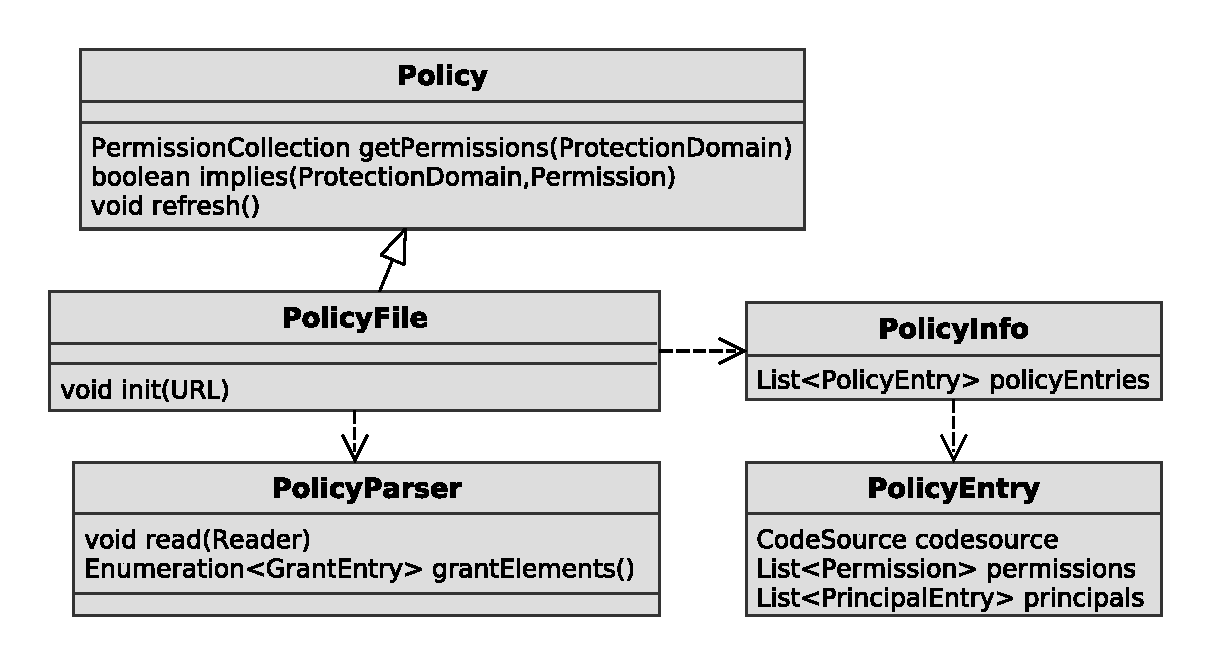
\includegraphics[width=14cm]{fig/policy-schema}
  \caption{Schéma tříd podílejících se na politice postavené na souboru politiky.}
\end{figure}

Standardní implementace bezpečnostní politiky {\it PolicyFile} využívá {\it PolicyParser} pro převod jednotlivých textových bloků {\it grant} do objektové podoby.
Takto získaný výčet objektů {\it GrantEntry} pak převádí na seznam objektů {\it PolicyEntry}, které ukládá do atributu {\it policyEntries} objektu vnitřní třídy {\it PolicyFile.PolicyInfo}.

%,,,,,,,,,,,,,,,,,,,,,,,,,,,,,,,,,,,,,,,,,,,,,,,,,,,,,,,,,,,,,,,,,,,,,,,,,,,,,
\subsubsection{Příklad souboru bezpečnostní politiky}
%'''''''''''''''''''''''''''''''''''''''''''''''''''''''''''''''''''''''''''''

Tento příklad ukazuje jednoduchou bezpečnostní politiku, opět v kontextu příkladu knihovny pro přístup k databázi z kapitoly \ref{databazeVsouboru}.

\begin{verbatim}
grant codeBase "file:/srv/program/" {
  permission ZaznamPermission "Lucka", "nacteni";
};
grant codeBase "file:/srv/knihovna/" {
  permission ZaznamPermission "*", "nacteni";
  permission java.io.FilePermission "/srv/knihovna/data/-","read,write";
};
\end{verbatim}

Programu zde má přiděleno oprávnění k načtení záznamu "Lucka", nemůže ale přistupovat k s samotným databázovým souborů. K těmto má oprávnění přistupovat jen knihovna zpřístupňující tuto databázi. Kvůli způsobu implementace kontroly oprávnění Access controllerem (popsaným v kapitole \ref{implementaceAC}) je nezbytné přidělit knihovně oprávnění ke všem záznamům v databázi, jinak by žádná kontrola oprávněnosti požadavku nemohla skončit pozitivně.

%,,,,,,,,,,,,,,,,,,,,,,,,,,,,,,,,,,,,,,,,,,,,,,,,,,,,,,,,,,,,,,,,,,,,,,,,,,,,,
\subsubsection{Zástupné znaky}
%'''''''''''''''''''''''''''''''''''''''''''''''''''''''''''''''''''''''''''''

URL kořene systému balíčků může být ukončeno zástupnými znaky pomlčka ({\tt -}) a hvězdička ({\tt *}).

Zatímco {\tt /*} odpovídá všem souborům v daném adresáři, {\tt /-} odpovídá všem souborům v daném adresáři i jeho podadresářích, rekurzivně. V obou případech jsou zahrnuty jak soubory tříd ({\tt .class}), tak i celé archivy tříd ({\tt .jar}/{\tt .war}/{\tt .ear}).
\cite{jdkdocPolicyFiles}

%-----------------------------------------------------------------------------
\subsection{Nastavení souboru a třídy bezpečnostní politiky}\label{souborPolitiky}
%-----------------------------------------------------------------------------

Nastavení souboru a třídy bezpečnostní politiky umožňuje správci nebo uživateli počítače stanovit bezpečnostní politiku aplikovanou na programy v Javě běžící na tomto počítači bez potřeby znalostí programování.

Toto nastavení se provádí úpravou konfiguračního souboru {\it java.security}, jehož přesné umístění je platformně závislé. Typicky je v umístění {\it \$JRE\_HOME/lib/security/java.policy} pro celý systém, nebo v umístění {\it \$USER\_HOME/.java.policy} pro jednotlivé uživatele. \cite{refSecurity}
Jeho význačnější proměnné jsou: \cite[5.3.1]{oaks}

\begin{verbatim}
policy.provider=sun.security.provider.PolicyFile
policy.url.1=file:${java.home}/lib/security/java.policy
policy.url.2=file:${user.home}/.java.policy
\end{verbatim}

V tomto souboru lze tedy globálně nastavit používanou třídu bezpečnostní politiky a adresu standardně používaného souboru bezpečnostní politiky pro celý systém nebo uživatele systému, pod kterým JVM běží.

Bezpečnostní politiku je dále možné rozšířit při startu JVM o vlastní soubor bezpečnostní politiky úpravou konfigurační proměnné parametrem příkazu, jímž program budeme spouštět: \cite[5.3.1]{oaks}

\begin{verbatim}
java -Djava.security.policy=dalsi_soubor_politiky.policy ProgramABC
\end{verbatim}

V tomto případě bude uvedený soubor bezpečnostní politiky použit zároveň s výše uvedeným standardním souborem bezpečnostní politiky. Chceme-li standardní soubor bezpečnostní politiky zcela nahradit, stačí namísto rovnítka v definici konfigurační proměnné použít rovnítka dvě: \cite[5.3.1]{oaks}

\begin{verbatim}
java -Djava.security.policy==jediny_soubor_politiky.policy ProgramABC
\end{verbatim}

Obsah této konfigurační proměnné je možné změnit také za běhu programu, má-li daná část programu potřebná oprávnění:

\begin{verbatim}
System.setProperty("java.security.policy", "jiny_soubor_politky.policy");
\end{verbatim}

Tato konfigurační proměnná je čtena při inicializaci Access controlleru. Na jejím základě je následně soubor bezpečnostní politiky načten a aplikován. Chceme-li soubor bezpečnostní politiky vyměnit za běhu, pouhá změna obsahu této konfigurační proměnné proto nestačí -- je třeba zapříčinit nové načtení souboru bezpečnostní politiky. K tomuto účelu je možné použít metodu třídy {\it Policy}, která právě toto provádí:

\begin{verbatim}
Policy.getPolicy().refresh();
\end{verbatim}

Problémem je, že tato metoda je označena jako nedoporučovaná ({\it deprecated}), protože je implementačně závislá -- zatímco u implementace používající soubory bezpečnostní politiky správně způsobí projevení změn v souboru bezpečnostní politiky, u jiných implementací bezpečnostní politiky může být implementována jako prázdná operace. Navíc i v případě různých implementací politiky založené na souborech se může chovat odlišně, například v závislosti na strategii vyrovnávací paměti kolekce oprávnění ({\it PermissionCollection}) -- může znovu načíst bezpečnostní politiku pro celou JVM, ale také třeba jen pro danou ochranou doménu. \cite{refPolicy}

Tato práce se proto bude zabývat jen bezpečnostními politikami poskytovanými standardní implementací třídy {\it Policy} -- {\it sun.security.provider.PolicyFile}.

%%%%%%%%%%%%%%%%%%%%%%%%%%%%%%%%%%%%%%%%%%%%%%%%%%%%%%%%%%%%%%%%%%%%%%%%%%%%%%
\chapter{Distribuované prostředí Red Hat JBoss}
%%%%%%%%%%%%%%%%%%%%%%%%%%%%%%%%%%%%%%%%%%%%%%%%%%%%%%%%%%%%%%%%%%%%%%%%%%%%%%

WildFly, dříve známý jako JBoss AS, je aplikační server standardu Java EE. Poskytuje tedy běhové prostředí Java EE aplikacím, které se na tento aplikační server nainstalují.

Instalace WildFly je možné spojit do domény a vytvořit tak distribuované prostředí. Každou instalaci WildFly pak nazýváme hostitelem. Doména je tedy skupinou hostitelů ({\it host}), přičemž na jediném počítači může teoreticky běžet více hostitelů. Typicky však jeden hostitel odpovídá jednomu počítači.

Jeden z hostitelů plní funkci doménového řadiče ({\it domain controller}). Tento hostitel je nositelem jediného používaného konfiguračního souboru domény, {\it domain.xml}. Každý z hostitelů je konfigurován svým konfiguračním souborem {\it host.xml}, jež určuje, zda-li je hostitel doménovým řadičem nebo, v případě že doménovým řadičem není, adresu doménového řadiče, na který by se tento hostitel měl registrovat. \cite{jbossDomainSetup}

Na každém hostiteli může běžet více serverů -- instancí aplikačního serveru běžících ve vlastních JVM. Každý server má vlastní jméno, jímž se registruje v doméně, sadu portů na kterých poskytuje své služby a JVM ve které běží. Vše z uvedeného je přitom součástí definice serveru v konfiguračním souboru hostitele, {\it host.xml}. \cite{jbossDomainSetup}

Server je také zařazen do jedné ze skupin serverů, jež jsou definovány v konfiguračním souboru domény. Přiřazení serveru do skupiny je součástí definice serveru v konfiguračním souboru hostitele. \cite{jbossDomainSetup}

Skupiny serverů tedy seskupují servery napříč hostiteli s některými společnými vlastnostmi -- aplikace (deployment) je typicky nasazována na celou skupinu serverů najednou a konfigurace skupiny umožňuje provést nastavení (např. nastavit parametr JVM) na všech serverech skupiny najednou. \cite{jbossDomainSetup}

%=============================================================================
\section{Běh WildFly pod Java Security Managerem}
%=============================================================================

Nakonfigurovat použití security manageru na aplikační server WildFly je možné stejně jako na jakoukoli jinou aplikaci v Javě -- nastavením patřičných konfiguračních vlastností popsaných v kapitolách \ref{souborPolitiky} a \ref{securityManager} při startu JVM. To je nejjednodušeji možné zajistit parametrem {\it -D} příkazu {\it java}. Ve spouštěcím skriptu WildFly ({\it standalone.sh} / {\it domain.sh} / {\it standalone.bat} / {\it domain.bat}) je pro tyto potřeby používána proměnná {\it JAVA\_OPTS}. Připojením parametrů na konec této proměnné tak dosáhneme nastavení použití security manageru a bezpečnostní politiky ve všech JVM aplikačního serveru: \cite{jbossSecurityManager}

\begin{verbatim}
JAVA_OPTS="$JAVA_OPTS -Djava.security.manager"
JAVA_OPTS="$JAVA_OPTS -Djava.security.policy==directory/wildfly.policy"
\end{verbatim}

Jestliže budeme dále předpokládat, že cílem nasazení bezpečnostních politik na server je omezení možností uživatelských aplikací, můžeme od jemného přidělování jen nejnezbytnějších oprávnění součástem WildFly které je nezbytně potřebují, ustoupit k přidělení všech oprávnění všem součástem aplikačního serveru. Uživatelské aplikace nyní ponecháme bez jakýchkoli oprávnění a vyzkoušíme účinky této bezpečnostní politiky:

\begin{verbatim}
grant codeBase "file:${jboss.home.dir}/jboss-modules.jar" {
    permission java.security.AllPermission;
};
grant codeBase "file:${jboss.home.dir}/modules/-" {
    permission java.security.AllPermission;
};
\end{verbatim}

S použitím této bezpečnostní politiky server WildFly skutečně bez problému nastartuje. Když však na tento server nasadíme aplikaci provádějící kupříkladu čtení souboru uloženého v adresáři této aplikaci, zjistíme že aplikace nemá problém tento soubor číst. Do souboru ležícího mimo jeho adresář se ale naopak nedostane dokonce ani pokud toto oprávnění benevolentně přidělíme všem programům v JVM bez ohledu na jejich kořen balíčků ({\it codeBase}).

Protože použijeme-li naopak prázdný soubor bezpečnostní politiky, start server se nezdaří, je očividné že bezpečnostní politika byla nastavena správným způsobem, ale po startu aplikačního serveru byla aplikačním serverem nahrazena.

%Na základě znalostí uvedených v kapitole \ref{teoretickyUvod} jsem příčinu hledal \cite{javaEEspec}

{\it TODO }



%=============================================================================
\section{Security manager WildFly}
%=============================================================================








%%%%%%%%%%%%%%%%%%%%%%%%%%%%%%%%%%%%%%%%%%%%%%%%%%%%%%%%%%%%%%%%%%%%%%%%%%%%%%
\chapter{Návrh systému}
%%%%%%%%%%%%%%%%%%%%%%%%%%%%%%%%%%%%%%%%%%%%%%%%%%%%%%%%%%%%%%%%%%%%%%%%%%%%%%

Cílem práce je vytvoření systému pro centralizovanou správu a distribuci bezpečnostních politik. Měl by umožnit nasazovat bezpečnostní politiky na jednotlivé servery domény WildFly a sledovat také, které bezpečnostní politiky jsou právě na kterých serverech domény WildFly nasazeny.

Jako příhodné se pro tento účel zdá využití rozšiřitelnosti systému WildFly a implementace zmíněné funkcionality formou subsystému aplikačního serveru WildFly. Subsystém je rozšířením aplikačního serveru a jeho konfigurace i přítomnost je nastavována zvlášť pro každý profil, přičemž profil je souhrnem konfigurace serveru a je nastavovaný pro celé skupiny serverů. Optimálním řešením by bylo takové rozšíření WildFly, jež by bylo nasazováno a konfigurováno nezávisle na profilech jednotlivých serverů. Takový koncept ale bohužel WildFly neposkytuje.

Nadále proto budeme předpokládat, že všechny skupiny serverů, v rámci kterých chceme s bezpečnostními politikami manipulovat, používají stejný konfigurační profil.

%=============================================================================
\section{Způsob nastavení bezpečnostní politiky}
%=============================================================================

Uživatel i aplikace mohou se subsystémem komunikovat prostřednictvím JBoss native management API. To je navrženo pro maximální jednoduchost a k nejrůznějším nastavením, které by jinak byly reprezentovány objekty velkého množství tříd, je možné přistupovat jako ke stromu objektů obecných tříd uzel ({\it ModelNode}) a vlastnost (Property). Uzly tvoří strom a každý uzel může mít vlastnosti, jež obsahují samotnou konfiguraci aplikačního serveru ve formě textových řetězců ({\it String}), do kterých tedy musí být převedeny i hodnoty jiných datových typů. \cite{jbossDetypedManagement}

Klient JBoss native management API, kterým jsou zejména CLI rozhraní WildFly a Webová konzola WildFly, tedy musí implementovat jen práci s tímto konfiguračním stromem. Jeho implementace tedy teoreticky nemusí vůbec záviset na typu informace v konfiguračním stromu. V praxi toto ale pochopitelně platí jen pro nízkoúrovňové nástroje sloužící k přímé úpravě konfiguračního stromu, jakým je CLI rozhraní WildFly. Webová konzola naproti tomu pracuje s více konkrétními třídami objektů, jakými jsou server, skupina ({\it server-group}) nebo zdroj dat ({\it datasource}). Přestože pracuje se stejným konfiguračním stromem, tvořeným jen těmito dvěma datovými typy, je závislá na struktuře kterou uzly tohoto stromu tvoří. Jednoduchost JBoss native management API je tak znatelná spíše jen na stabilitě tohoto API a knihovně pro práci s ním -- {\it jboss-dmr}. \cite{jbossDetypedManagement}

Rozšíření aplikačního serveru, kterým je například subsystém, vykonává svůj kód zejména v reakci na události, které si zaregistruje. Těmito událostmi bývá zpravidla načtení rozšíření a přidání a odebrání subsystému, často také operace nad uživatelským balíčkem (nasazení apod.) nebo právě operace nad definovanou konfigurační vlastností. \cite{WildFlyExtending}

Jako vhodné řešení bylo tedy zvoleno nasazení bezpečnostní politiky v návaznosti na nastavení hodnoty konfigurační proměnné. Každý server aplikačního serveru bude mít v konfiguračním stromu svůj uzel a jeho vlastnostmi bude bude určen soubor bezpečnostní politiky, jež by měl být nasazený na daném serveru a také to, zda by měl být security manager pro daný server vůbec zapnutý.

Samotná operace provedení výměny bezpečnostní politiky a případného zapnutí/vypnutí security manageru pak bude spojena s událostí nastavení hodnoty dané vlastnosti. Vlastnosti bude přiřazena metoda, jež má být volána při zápisu do její hodnoty. Ta zajistí výměnu bezpečnostní politiky prostřednictvím k tomu určené třídy, jež bude součástí vytvářeného subsystému.

%=============================================================================
\section{Způsob šíření souborů bezpečnostní politiky} \label{sireniSouboru}
%=============================================================================

Jelikož cílem práce není jen centralizovaná správa, ale i distribuce bezpečnostních politik, je nutné rovněž stanovit způsob, jakým soubory bezpečnostní politiky budou šířeny mezi servery WildFly domény.

Jako pravděpodobně nejjednodušší řešení, které by bylo možné navrhnout, lze označit vytvoření sdíleného adresáře, jež by byl přístupný z každého serveru domény, například protokolem NFS (Network File System).

S tímto řešením však souvisí hned několik potíží. První z nich je vyšší platformní závislost -- zatímco WildFly jakožto aplikace v Javě bez problému běží na mnoha platformách a pod různými operačními systémy, protokol NFS není napříč operačními systémy příliš podporován. Tento problém by bylo možné řešit použitím více rozšířeného protokolu umožňujícího vzdálený přístup k souborům, jakým je například FTP.

Druhým problém je ale bezpečnost -- protokoly FTP ani NFS samy o sobě nedokáží zaručit autenticitu serveru, ke kterému se klient připojuje. Případný útočník by se tak mohl vydávat za FTP/NFS server na němž jsou bezpečnostní politiky uložené a podvrhnout tak serverům domény vlastní bezpečnostní politiky. Tento problém by mohlo vyřešit použití lépe zabezpečeného protokolu, jakým je například SSH (Secure Shell), jež umožňuje vzdálený přístup k souborům prostřednictvím SSHFS (SSH Filesystem), nebo FTPS (FTP over SSL), kde se server vůči klientovi autentizuje za pomoci asymetrické kryptografie. \cite[3]{ssh}

Použití těchto lépe zabezpečených protokolů zajistí bezpečnost systému, avšak umocní problém platformních omezení, obzvláště v případě protokolu SSH. Navíc i v případě dokonalého zajištění sdíleného adresáře bezpečnostních politik bude nutné zajistit také bezpečný přenos informací po JBoss Native API, pro bezpečný přenos informace, kterou bezpečnostní politiku má daný server použít.

Problém bezpečnosti distribuce bezpečnostních politik je možné si představit jako řetěz. Řetěz je jen tak silný, jak silný je jeho nejslabší článek. Aby byl řetěz silný, je třeba mít silné všechny jeho články -- v tomto případě bezpečnost komunikačního kanálu, po kterém se přenáší soubory bezpečnostních politik a komunikačního kanálu, po kterém se přenáší informace, který soubor bezpečnostní politiky by měl daný server použít.

Touto úvahou lze dojít k závěru, že optimálním řešením je minimalizovat počet článků řetězu -- sloučit tyto dva komunikační kanály do jediného a nadále řešit bezpečnost jen tohoto jediného komunikačního kanálu.

Toto lze implementovat za pomoci uzlů konfiguračního stromu jednotlivých politik představujících jednotlivé soubory politik. Vlastností tohoto uzlu by pak obsah samotného souboru bezpečnostní politiky. Soubory bezpečnostní politiky by pak mohly být nahrávány do těchto vlastností konfiguračních uzlů na straně doménového řadiče a naopak z nich čteny na straně ostatních členských serverů WildFly domény.

Protože však použití standardní třídy bezpečnostní politiky ({\it sun.security.provider.PolicyFile}) vyžaduje soubory bezpečnostní politiky přístupné skrze URL adresu souboru, je na straně členských serverů třeba před aplikací bezpečnostní politiky obsah souboru bezpečnostní politiky zapsat do dočasného souboru.

Protože bude tento postup nezbytné aplikovat na straně členských serverů domény, je zbytečné řešit toto na doménovém řadiči jinak. Ztrácí se tak také většina důvodů pro to, aby byly bezpečnostní politiky na straně doménového řadiče uloženy v souboru souborového systému.

Jako výhodnějším řešením se tedy začíná jevit ukládat bezpečnostní politiky přímo do vlastností konfiguračních uzlů. Tím bude vyřešen i problém, jak ze strany aplikačního serveru detekovat, že byl soubor bezpečnostní politiky změněn. Zatímco v případě souboru by bylo nezbytné se periodicky dotazovat na čas poslední změny tohoto souboru, na změnu hodnoty konfigurační vlastnosti je možné navázat programovou událost, a tím zajistit aplikaci bezpečnostní politiky přímo v návaznosti na změnu hodnoty její konfigurační vlastnosti.

%=============================================================================
\section{Webové uživatelské rozhraní} \label{navrhGUI}
%=============================================================================

Součástí zadání práce bylo také vytvořit webové rozhraní pro komunikaci s uživatelem. Jelikož je samotné jádro řešení implementováno jako subsystém WildFly, jako optimální řešení se nabízí implementovat uživatelské rozhraní tohoto subsystému jako rozšíření webové konzoly WildFly.

Webová konzola WildFly je standardní součástí aplikačního serveru WildFly. Je GWT aplikací běžící na straně klienta, ve webovém prohlížeči, a se serverem komunikuje prostřednictvím HTTP Management API. To je alternativou Native API -- plní stejnou funkci, ale běží nad protokolem HTTP. Tělem odpovědí serveru i tělem POST dotazů klienta je JSON reprezentace uzlu konfiguračního stromu ({\it ModelNode}). \cite{WildFlyManagementAPIreference}

\begin{figure}[ht]
  \centering
  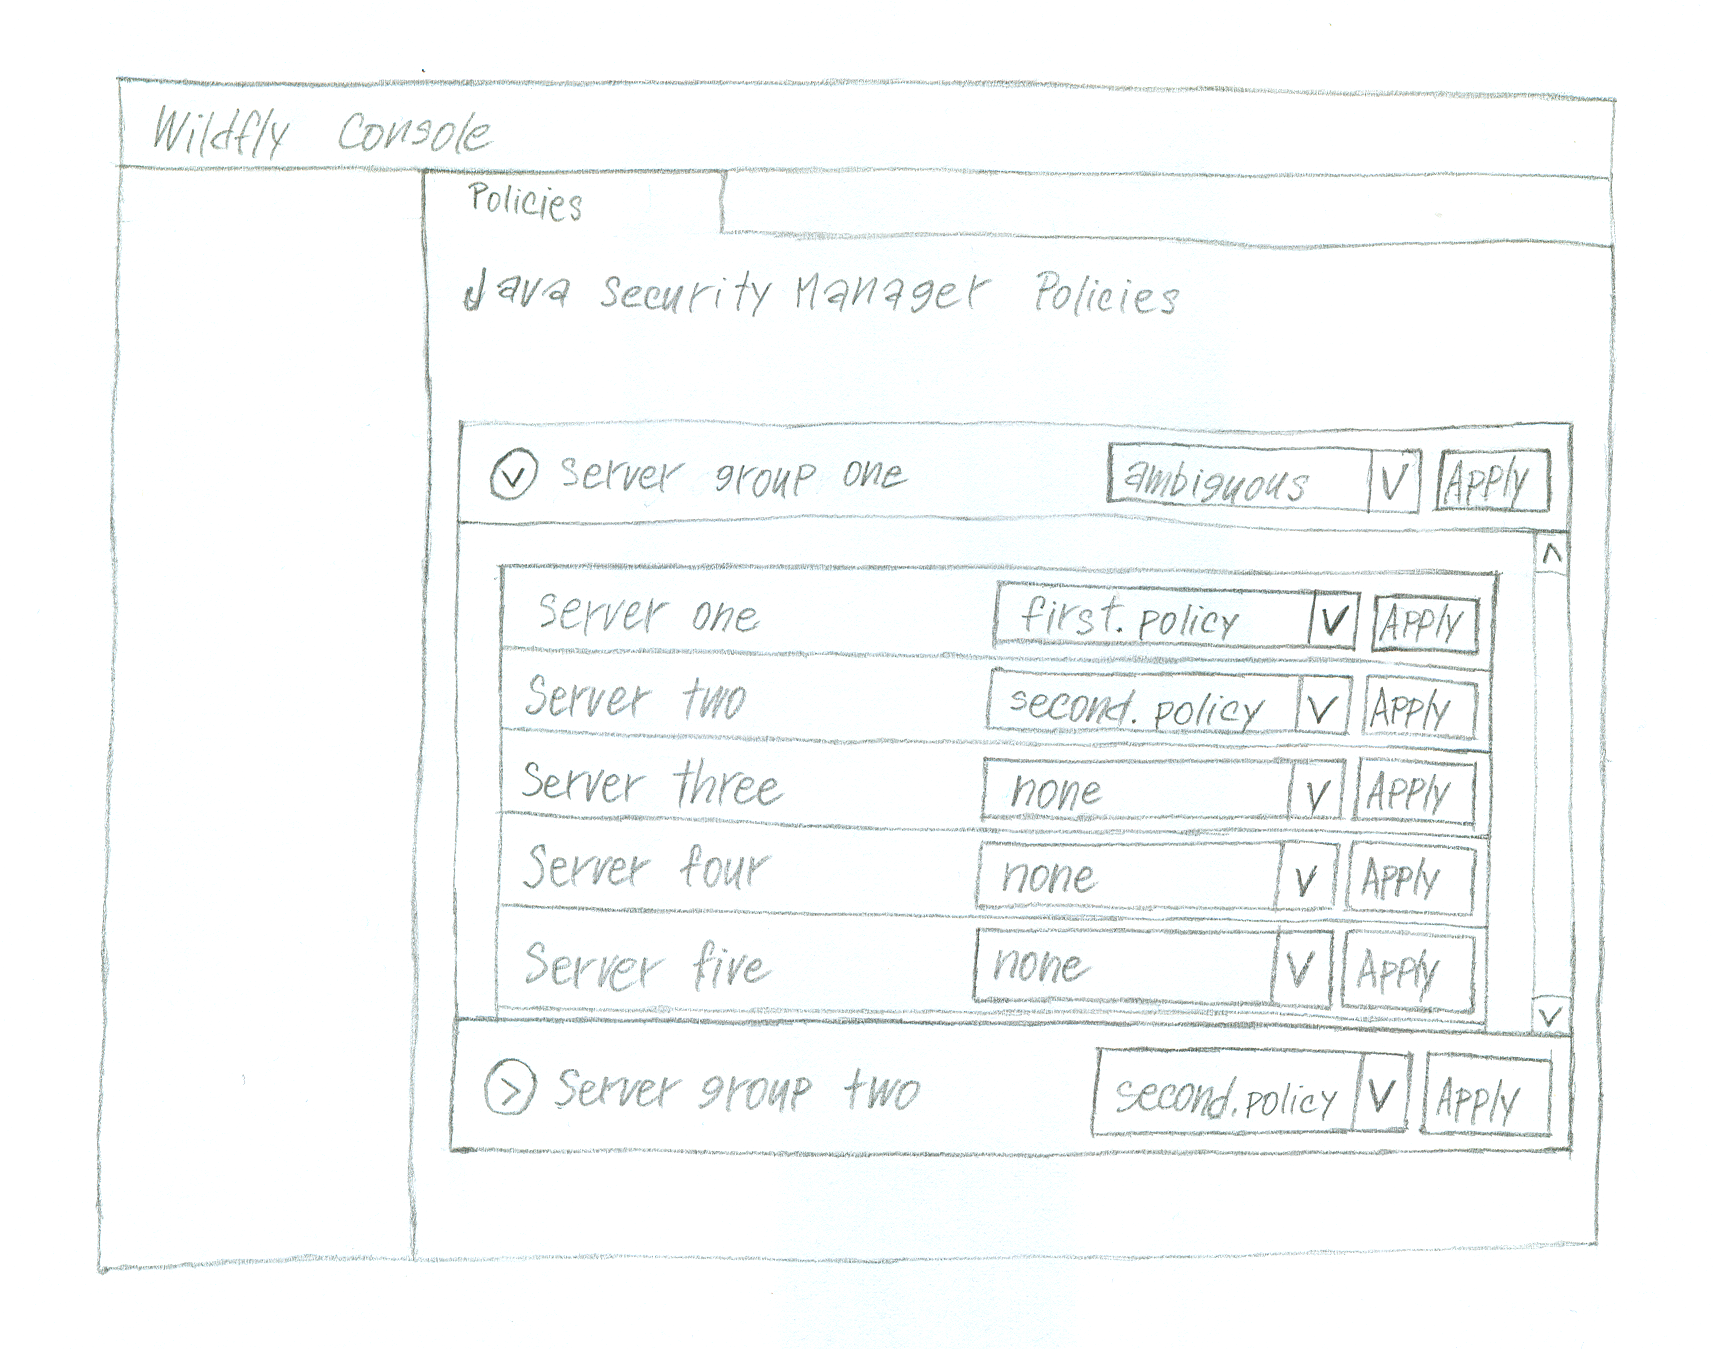
\includegraphics[width=14cm]{fig/mockup}
  \caption{Grafický návrh uživatelského rozhraní plánovaného rozšíření WildFly.}
\end{figure}

%%%%%%%%%%%%%%%%%%%%%%%%%%%%%%%%%%%%%%%%%%%%%%%%%%%%%%%%%%%%%%%%%%%%%%%%%%%%%%
\chapter{Popis implementace systému} \label{implementace}
%%%%%%%%%%%%%%%%%%%%%%%%%%%%%%%%%%%%%%%%%%%%%%%%%%%%%%%%%%%%%%%%%%%%%%%%%%%%%%

%=============================================================================
\section{První etapa}
%=============================================================================

V rámci první etapy implementace řešení byl implementován jednoduchý subsystém WildFly za pomoci kostry subsystému z Maven repozitáře, podle dokumentace WildFly 8 věnující se právě vytváření rozšíření WildFly. \cite{WildFlyExtending}

Dle tohoto vzoru byl vytvořen subsystém, jehož jedinou funkcí bylo rozšíření konfiguračního stromu o uzly server=* uchovávající informaci o URL bezpečnostních politik, jež by měly být uloženy na jednotlivých serverech domény WildFly odpovídajících svým jménem jménu tohoto konfiguračního uzlu. Tyto uzly fungovaly jako běžné uzly konfiguračního stromu WildFly -- administrátor měl možnost je vytvářet, odstraňovat a nastavovat jejich vlastnost {\it policy}, jež nesla právě samotnou URL nasazené bezpečnostní politiky.

Na změnu této konfigurační vlastnosti zároveň server domény daný jménem uzlu reagoval právě nasazením dané bezpečnostní politiky, prostřednicvím registrace této události při tvorbě konfigurační vlastnosti {\it policy} uzlu {\it server=*}.

Toho bylo dosaženo vytvořením třídy {\it ServerWriteAttributeHandler} a jejím uvedením v rámci volání provádějícího registraci samotné konfigurační vlastnosti:

\begin{verbatim}
resourceRegistration.registerReadWriteAttribute(POLICY,
                null, ServerWriteAttributeHandler.INSTANCE);
\end{verbatim}

Není stanovena třída (na místě {\it null}) zprostředkovávající čtení tohoto konfigurační vlastnosti. Na čtení této vlastnosti není totiž vázána žádná akce, ani není nutné obsah vracený jako odpověď na pokus o čtení vlastnosti nikterak upravovat a je možné uživatele nechat číst samotnou vlastnost přímo.

Aby byla bezpečnostní politika aplikována nejen na základě akce administrátora, ale také automaticky po startu serveru, byla její aplikace navázána také na akci přidání nového uzlu {\it server=*}. Odstranění takového uzlu pak bude navázáno na odebrání bezpečnostní politiky, stejně jako kdyby byla vlastnost policy nastavena na nedefinovanou.

Obě akce je jsou implementovány jako třídy {\it ServerAdd} a {\it ServerRemove}, jež jsou na uzly typu {\it server=*} navázány skrze parametry konstruktoru třídy definující tento uzel konfiguračního stromu:

\begin{verbatim}
public class ServerDefinition extends SimpleResourceDefinition {
    private ServerDefinition() {
        super(JsmPolicyExtension.SERVER_PATH,
                JsmPolicyExtension.getResourceDescriptionResolver("server"),
                ServerAdd.INSTANCE,
                ServerRemove.INSTANCE);
    }
}
\end{verbatim}

Konfigurační uzly {\it server=*} jsou ukládány do konfiguračního XML souboru domény WildFly, jak je u konfigurační uzlů WildFly běžné. Ukládání veškeré konfigurace subsystému je implementováno ve třídě {\it SubsystemParser}.

%=============================================================================
\section{Druhá etapa}
%=============================================================================

V rámci druhé etapy bylo uživatelské rozhraní pozměněno dle grafického návrhu předvedeného v kapitole \ref{navrhGUI}. V souvislosti s touto změnou bylo nutné rozšířit rovněž subsystém WildFly. Jeho dosavadní implementace neumožňovala výběr bezpečnostní politiky formou výběru v rozbalovací nabídce.

Výběr formou rozbalovací nabídky vyžaduje od aplikace zobrazující nabídku znalost voleb, mezi nimiž může uživatel provádět výběr. To při dosavadní implementaci subsystému možné nebylo, neboť aplikace běžící na straně webového prohlížeče měla přístup k souborům (tedy i souborům bezpečnostních politik) možný jen právě prostřednictvím subsystému, který doposud přístup k seznamu souborů bezpečnostních politik neumožňoval.

Do konfiguračního stromu subsystému tak vedle dosavadních uzlů {\it server=*} popsaných v minulé podkapitole přibyly uzly {\it policy=*}, jež reprezentovaly právě jednotlivé soubory bezpečnostní politiky, jež bylo možné jako bezpečnostní politiky jednotlivých serverů nastavit. Tyto uzly nebyly ukládány do konfiguračního XML souboru aplikačního serveru, ale byly vytvářeny ze seznamu souborů nacházejících se v k tomu určeném adresáři aplikačního serveru.

Toto načítání seznamu souborů nebylo řešeno cestou ideální, za kterou by šlo nejspíše považovat přímé navázání jakéhokoli pokusu o čtení těchto konfiguračních uzlů na programovou obsluhu, jež by umožnila jako přímý výsledek tohoto dotazu vrátit přímo aktuální seznam souborů v adresáři bezpečnostních politik.

Vzhledem k ranosti této verze a odstranění těchto schopností systému v pozdějších etapách vývoje bylo načtení seznamu souborů bezpečnostních politik řešeno přímým vytvořením těchto konfiguračních uzlů při startu aplikačního serveru na základě obsahu adresáře bezpečnostních politik ve chvíli startu aplikačního serveru.

Hlavní nevýhodou tohoto přístupu byla přetrvávající potřeba zajištění přístupu k souborům bezpečnostních politik uložených na doménovém řadiči, nikoli však již na jednotlivých aplikačních serverech domény. Adresář bezpečnostních politik tak bylo nutné napříč aplikačními servery distribuovat jinou cestou. (Podrobněji popsanou v kapitole \ref{navrhGUI} zabývající se návrhem právě způsobu šíření souboru bezpečnostních politik.)

Později odhaleným nedostatkem se pak stal fakt, že do konfigurační vlastnosti {\it policy} byla ukládána absolutní cesta k souboru bezpečnostní politiky, což by výrazně zkomplikovalo ostré nasazení implementovaného systému.

%=============================================================================
\section{Třetí etapa}
%=============================================================================

V rámci třetí etapy implementace byl subsystém WildFly upraven, aby konfigurační strom WildFly nefungoval jen jako úložiště adres nastavených bezpečnostních politik, ale také jako úložiště samotných bezpečnostních politik.

Byl tedy pozměněn význam konfigurační vlastnosti {\it file} uzlu {\it policy=*}. Absolutní URL adresa souboru  bezpečnostní politiky byla nahrazena obsahem souboru bezpečnostní politiky.

Zároveň byl změněn význam konfigurační vlastnosti {\it policy} uzlu {\it server=*}, jež doposud rovněž obsahoval URL adresu souboru bezpečnostní politiky nasazené na daném serveru. Nově byl nahrazen jménem uzlu {\it policy=*}, jehož bezpečnostní politika z jeho vlastnosti {\it file} byla na daný server nově nasazována.

Nadále tak nestačilo provádět aplikaci bezpečnostní politiky při změně atributu {\it policy} uzlu {\it server=*}, ale bylo nutné bezpečnostní politiku používanou aplikačním serverem vyměnit rovněž při změně obsahu vlastnosti {\it file} uzlu {\it policy=*}.

Toto je řešeno analogicky jako právě v případě akce navázané na změnu vlastnosti uzlu serveru -- vytvořením třídy {\it PolicyWriteAttributeHandler} a jejím navázáním na vlastnost uzlu bezpečnostní politiky.

%%%%%%%%%%%%%%%%%%%%%%%%%%%%%%%%%%%%%%%%%%%%%%%%%%%%%%%%%%%%%%%%%%%%%%%%%%%%%%
\chapter{Testování systému}
%%%%%%%%%%%%%%%%%%%%%%%%%%%%%%%%%%%%%%%%%%%%%%%%%%%%%%%%%%%%%%%%%%%%%%%%%%%%%%

Protože cílem této bakalářské práce nebylo jen vytvoření systému umožňujícího správu bezpečnostních politik nasazených na jednotlivých serverech distribuovaného systému ale také jeho otestování, tato kapitola se zabývá vytvořením testů, umožňujících otestovat implementované řešení.

Testování je nedílnou součástí vývoje software a je užíváno k odhalení vad software a prokázání, že software dosáhl požadované úrovně kvality v zadaných kritériích. \cite{ivsTest}

Testování je možné dělit do tří kategorií:

\begin{enumerate}
  \item {\textbf Jednotkové testování (Unit testing)}, kde se testují jednotlivé součásti systému zvlášť, v izolaci od ostatních součástí systému -- součásti systému, na kterých testovaná součást závisí jsou během testu nahrazeny jejich napodobeninami. Cílem je odhalit odlišnosti ve fungování součásti oproti specifikaci. \cite{ivsTest}
  \item {\textbf Integrační testování (Integration testing)}, kde se testují celé podsystémy -- jednotlivé součásti systému ve spojení se součástmi, na kterých testovaná součást závisí. Cílem je odhalit chyby v propojení jednotlivých součástí a v jejich vzájemné interakci. \cite{ivsTest}
  \item {\textbf Systémové testování (System testing)}, kde se testuje celý systém jako celek. Cílem je odhalit odlišnosti v chování systému vůči jeho specifikaci. \cite{ivsTest}
\end{enumerate}


%=============================================================================
\section{Jednotkové testování (Unit testing)}
%=============================================================================

Jednotkové testy tedy umožňují testovat jednotlivé jednotky programu, kterými jsou typicky třídy. Každé třídě programu by pak měla být přidělena jedna třída testu, jež by měl ověřit korektnost chování této testované třídy.

Testované jednotky by při jednotkovém testovaní měly být testovány ve vzájemné izolaci. K tomuto účelu se obvykle využívají tzv. mock objekty -- objekty napodobující chování objektů jednotek, od kterých má být testovaná jednotka izolována.



%=============================================================================
\section{Integrační testování (Integration testing)}
%=============================================================================

Integrační testy testují jednotlivé jednotky programu bez jejich vzájemné izolace. Umožňují tak testovat jak samotné testované jednotky, tak i schopnost jejich vzájemné spolupráce.




%=============================================================================
\section{Systémové testování (System testing)}
%=============================================================================

Systém jako celek byl testován hlavně na schopnost plnění základních požadavků zadání práce -- schopnosti zapnout a vypnout security manager a vyměnit používanou bezpečnostní politiku.

K tomuto účelu byl vytvořen systémový test umožňující otestovat zmíněné schopnosti na běžícím aplikačním serveru WildFly s nainstalovaným subsystémem pro nastavení bezpečnostní politiky, jež byl vytvořen v minulé kapitole \ref{implementace}.

Tento test se skládá ze dvou částí -- agenta, aplikace nasazované na testovaný server, a manageru, testu vytvořeného za pomoci knihovny JUnit, řídícího proces samotného testování.

Agent je Java EE aplikací nabízející své služby skrze rozhraní REST. Službami, jež poskytuje, je zejména otestování schopnosti provést vybranou akci z pozice aplikace nasazené na testovaném serveru. Klient rozhraní REST se tedy k této službě může připojit a požádat o otestování schopnosti provést vybranou operaci. Jako odpověď pak dostane informaci, zda-li se provedení této operace zdařilo, nebo zda bylo zmařeno Access controllerem.

Mimo toho tato služba umožňuje manageru zjistit také některé další informace o aplikačním serveru, zjistitelné ze strany aplikace nasazené na tomto aplikačním serveru, jako je aktuálně používaná třída security manageru, používaná třída bezpečnostní politiky, nebo samotná přítomnost agenta na testovaném aplikačním serveru.

Manager je část systémového testu běžící mimo aplikační server. Sestává z testů založených na knihovně JUnit a pomocných tříd {\it Domain} a {\it Server}.

Třída {\it Server} zajišťuje komunikaci manageru s agentem nasazeným na testovaném serveru WildFly prostřednictvím protokolu REST. Některé testy, například testy vzájemného ovlivňování serverů mezi sebou, mohou vyžadovat monitoring více serverů WildFly najednou. Na každém z nich pak musí být nasazena aplikace agenta a s každým z nich pak bude moci test komunikovat prostřednictvím samostatné instance třídy {\it Server}.

Třída {\it Domain} mezitím zajišťuje komunikace se samotnou doménou aplikačních serverů prostřednictvím protokolu JBoss Native API. Umožňuje manipulovat s konfiguračním stromem WildFly, zejména přidávat a upravovat hodnoty konfiguračních vlastností uzlů {\it server=*} a {\it policy=*} a tím nasazovat bezpečnostní politiky na jednotlivé servery WildFly domény.

Určitý problém, jež bylo nutno vyřešit, zde představuje způsob, jakým po skončení každého testu navrátit systém do původního stavu. Jelikož se jedná o testování z vně aplikačního serveru, není pro tento účel možné využít operaci {\it rollback}, jež se běžně automaticky provádí při selhání objektu ošetřujícího událost úpravy konfiguračního uzlu.

Budeme-li však předpokládat že testy budou prováděny na k tomu určené doméně aplikačních serverů, můžeme pominout požadavek na navrácení původní konfigurace po ukončení testování a omezit navrácení do původního stavu na navrácení do stavu s prázdným konfiguračním uzlem subsystému, tedy bez jakýchkoli konfiguračních uzlů 
{\it server=*} nebo {\it policy=*}.

Další operací objektu domény tak bude navrácení subsystému do počátečního stavu. Toho bude dosaženo spojením operace odstranění uzlu subsystému {\it jsmpolicy} konfiguračního stromu a jeho opětovné přidání.

%%%%%%%%%%%%%%%%%%%%%%%%%%%%%%%%%%%%%%%%%%%%%%%%%%%%%%%%%%%%%%%%%%%%%%%%%%%%%%
\chapter{Závěr}
%%%%%%%%%%%%%%%%%%%%%%%%%%%%%%%%%%%%%%%%%%%%%%%%%%%%%%%%%%%%%%%%%%%%%%%%%%%%%%

Cílem práce bylo navrhnout, vytvořit a otestovat systém pro centralizovanou správu a distribuci bezpečnostních politik Javy v distribuovaném prostředí aplikačního serveru WildFly.


